\documentclass{standalone}
\usepackage{times}
\usepackage{mathtools}

\usepackage{tikz}
\usetikzlibrary{positioning,fit,shapes,calc,decorations.pathreplacing}
\usetikzlibrary{backgrounds}
\usetikzlibrary{arrows.meta}
\usetikzlibrary{shapes,snakes}

\definecolor{processblue}{cmyk}{1,1,1,0}
\definecolor{accent}{rgb}{0.6,0.6,0.6}
\definecolor{accent2}{rgb}{0.9,0.9,0.9}

\begin{document}
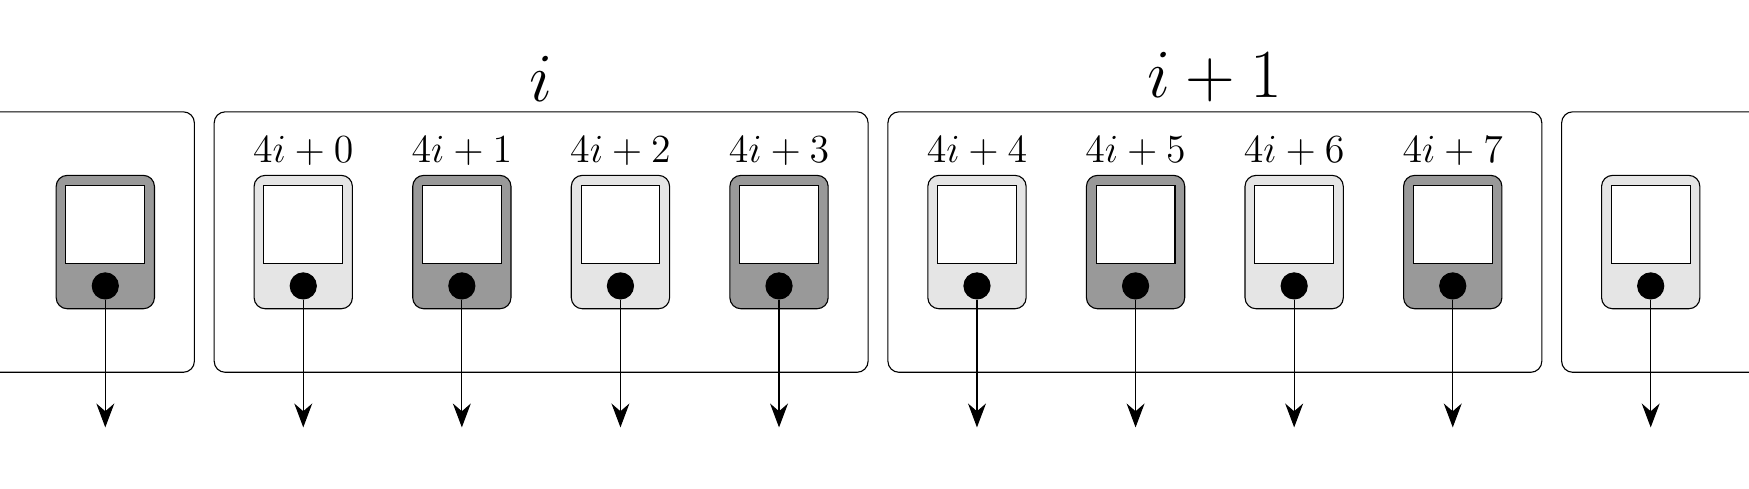
\begin{tikzpicture}[
  data/.style = {
    draw,
    rectangle,
    fill = white,
    minimum width = 1.0cm,
    minimum height = 1.0cm,
  },
  next/.style = {
    draw,
    circle,
    fill=black,
  },
  edge/.style = {
    draw,
    rectangle,
    rounded corners,
    minimum width = 0.5cm,
    minimum height = 0.5cm,
  },
  vedge/.style = {
    edge,
    top color = accent2,
    bottom color = accent2,
  },
  fedge/.style = {
    edge,
    top color = accent,
    bottom color = accent,
  },
  >={Stealth[scale=1.8]},
]

  \clip (-3.5,-3.0) rectangle (18,2.5);
  
  \node[data] (d0) {};
  \node[data] (d1) [right=of d0] {};
  \node[data] (d2) [right=of d1] {};
  \node[data] (d3) [right=of d2] {};

  \node[data] (d4) [right=1.5cm of d3] {};
  \node[data] (d5) [right=of d4] {};
  \node[data] (d6) [right=of d5] {};
  \node[data] (d7) [right=of d6] {};

  \node[data] (dl0) [left=1.5cm of d0] {};
  \node[data] (dl1) [left=of dl0] {};
  \node[data] (dr0) [right=1.5cm of d7] {};
  \node[data] (dr1) [right=of dr0] {};

  \node[next] (n0) [below=0.1cm of d0] {};
  \node[next] (n1) [below=0.1cm of d1] {};
  \node[next] (n2) [below=0.1cm of d2] {};
  \node[next] (n3) [below=0.1cm of d3] {};
  \node[next] (n4) [below=0.1cm of d4] {};
  \node[next] (n5) [below=0.1cm of d5] {};
  \node[next] (n6) [below=0.1cm of d6] {};
  \node[next] (n7) [below=0.1cm of d7] {};

  \node[next] (nl0) [below=0.1cm of dl0] {};
  \node[next] (nl1) [below=0.1cm of dl1] {};
  \node[next] (nr0) [below=0.1cm of dr0] {};
  \node[next] (nr1) [below=0.1cm of dr1] {};

  \begin{scope}[on background layer]
    \node[vedge,fit=(d0) (n0),label={\Large $4i+0$}] (e0) {};
    \node[fedge,fit=(d1) (n1),label={\Large $4i+1$}] (e1) {};
    \node[vedge,fit=(d2) (n2),label={\Large $4i+2$}] (e2) {};
    \node[fedge,fit=(d3) (n3),label={\Large $4i+3$}] (e3) {};
    \node[vedge,fit=(d4) (n4),label={\Large $4i+4$}] (e4) {};
    \node[fedge,fit=(d5) (n5),label={\Large $4i+5$}] (e5) {};
    \node[vedge,fit=(d6) (n6),label={\Large $4i+6$}] (e6) {};
    \node[fedge,fit=(d7) (n7),label={\Large $4i+7$}] (e7) {};

    \node[vedge,fit=(nl1) (dl1)] (el1) {};
    \node[fedge,fit=(nl0) (dl0)] (el0) {};
    \node[vedge,fit=(nr0) (dr0)] (er0) {};
    \node[fedge,fit=(nr1) (dr1)] (er1) {};
  \end{scope}
    
  \begin{scope}[on background layer]
    \node[draw,rectangle,fit=(e0) (e3),inner sep=0.5cm,inner ysep=0.8cm,rounded corners,label={\Huge $i$}] (q0) {};
    \node[draw,rectangle,fit=(e4) (e7),inner sep=0.5cm,inner ysep=0.8cm,rounded corners,label={\Huge $i+1$}] (q1) {};

    \node[draw,rectangle,fit=(el0) (el1),inner sep=0.5cm,inner ysep=0.8cm,rounded corners] (ql) {};
    \node[draw,rectangle,fit=(er0) (er1),inner sep=0.5cm,inner ysep=0.8cm,  rounded corners] (qr) {};
  \end{scope}

  \node (h0) [below=1.5cm of e0] {};
  \node (h1) [below=1.5cm of e1] {};
  \node (h2) [below=1.5cm of e2] {};
  \node (h3) [below=1.5cm of e3] {};
  \node (h4) [below=1.5cm of e4] {};
  \node (h5) [below=1.5cm of e5] {};
  \node (h6) [below=1.5cm of e6] {};
  \node (h7) [below=1.5cm of e7] {};

  \node (hl0) [below=1.5cm of el0] {};
  \node (hl1) [below=1.5cm of el1] {};
  \node (hr0) [below=1.5cm of er0] {};
  \node (hr1) [below=1.5cm of er1] {};

  \path[->] (n0) edge node {} (h0);
  \path[->] (n1) edge node {} (h1);
  \path[->] (n2) edge node {} (h2);
  \path[->] (n3) edge node {} (h3);
  \path[->] (n4) edge node {} (h4);
  \path[->] (n5) edge node {} (h5);
  \path[->] (n6) edge node {} (h6);
  \path[->] (n7) edge node {} (h7);

  \path[->] (nl0) edge node {} (hl0);
  \path[->] (nl1) edge node {} (hl1);
  \path[->] (nr0) edge node {} (hr0);
  \path[->] (nr1) edge node {} (hr1);

\end{tikzpicture}
\end{document}